%%%%%%%%%%%%%%%%%%%%%%%%%%%%%%%%%%%%%%%%%%%%%%%%%%%%%%%%%%%%%%%
%\subsection{Task 1}
%\label{sub:task1}
%%%%%%%%%%%%%%%%%%%%%%%%%%%%%%%%%%%%%%%%%%%%%%%%%%%%%%%%%%%%%%%

Task 1 comprises the generation of synthetic models (conforming the movie database metamodel~\cite{imdbcase}) from an input parameter $N \geq 0$. In the following we present an e-Motions based solution and a Maude solution. 


%%%%%%%%%%%%%%%%%%%%%%%%%%%%%%%%%%%%%%%%%%%%%%%%%%%%%%%%%%%%%%%
\subsubsection{e-Motions-based solution.}

Following an e-Motions based approach, we define the abstract and concrete syntax and the behavior of our so-called \textit{Task 1 DSL}. Taking a parameter $N$ as input model, \textit{Task 1 DSL} generates a model containing synthetic data.

As it has been introduced in Section~\ref{sub:emotions}, the abstract syntax of a DSL is given in e-Motions by means of a Ecore metamodel. In fact, this metamodel is provided beforehand in~\cite{imdbsources}. We call this metamodel \textit{Movies MM}. However, the \textit{parameter N} has to be modeled in some way, since in e-Motions the state is just a model. Hence, a new concept call \code{Parameter} has been added to Movies MM. This results in a so-called \textit{Movies* MM}. The class \code{Parameter} has two integer attributes \code{nP} and \code{nN}, positive graphs and negative graphs, due to data generation following Henshing graphs~\cite{henshing} is divided into positive and negative cases.

For the concrete syntax, Fig.~\ref{fig:concreteSyntax} shows how an image has been attached to each concept modeled in the Movies* MM. The behavior of this \textit{Task 1 DSL} is given by means of two in-place rules: \code{createPositive} and \code{createNegative}. Figure~\ref{fig:createPositive} shows the \code{createPositive} rule, which takes an object \code{p} of type \textit{Parameter} with \textit{nP} attribute greater or equal than $0$ and, after the rule application, synthetic data conforming to the Henshin rules~\cite{henshing} are created. Fig.~\ref{fig:createNegative} shows the \code{createNegative} rule, which is analogously defined.

Once the syntax and the behavior of the system has been coded, the user may specify a model, which conforms to \textit{Movies* MM}, containing an object \code{Parameter} with its two attributes \code{nP} and \code{nN} properly set. This model is used as initial model of the execution.

This solution is really close to the problem specification~\cite{imdbcase}. Both Fig.~\ref{fig:task1} and Fig.~2 in~\cite{imdbcase} specifying the data generation are almost the same. This solution demonstrates how close is the solution to the problem domain, and how user-friendly is e-Motions.

\subsubsection{Maude version.}
This proposal of Task 1 consists of a object-based Maude specification, which is composed by two main modules: the \code{MOVIES@MM} module defining the classes structure and the \code{TASK1} module defining the solution. The solution is coded using again two rules: \code{createPositive} and \code{createNegative}. One could realized that the Maude version is very much like the e-Motions version. In fact, the former is almost the textual version of the latter. Listing~\ref{lst:createPositive} shows the \code{createPositive} Maude rule that takes the \code{createPositive(N:Nat)} message and a \code{freshOid} auxiliary message---used to create new object identifiers---and returns such a object configuration conforming the Henshin specification~\cite{imdbcase}.

The messages \code{createPositive} and \code{createNegative} are generated in zero-rewrite steps with the equation showed in Listing~\ref{lst:createexampleeq}.

\begin{lstlisting}[caption=\code{createPositive} Maude rule., label=lst:createPositive]
rl [createPositive] :
  createPositive(N)
  freshOid(N')
=>
  < N'     : Movie | rating : (10.0 * float(N)) >
  < N' + 1 : Movie | rating : (10.0 * float(N) + 1.0) >
  < N' + 2 : Movie | rating : (10.0 * float(N) + 2.0) >
  < N' + 3 : Movie | rating : (10.0 * float(N) + 3.0) >
  < N' + 4 : Movie | rating : (10.0 * float(N) + 4.0) >
  
  < N' + 5 : Actor | name : ("a" + string((10 * N),     10)),
                   movies : (N', N' + 1, N' + 2, N' + 3)     >
  < N' + 6 : Actor | name : ("a" + string((10 * N + 1), 10)),
                   movies : (N', N' + 1, N' + 2)             >
  < N' + 7 : Actor | name : ("a" + string((10 * N + 2), 10)),
                   movies : (N' + 1, N' + 2, N' + 3)         >
  < N' + 8 : Actress | name : ("a" + string((10 * N + 3), 10)),
                   movies : (N' + 1, N' + 2, N' + 3, N' + 4) >
  < N' + 9 : Actress | name : ("a" + string((10 * N + 4), 10)),
                   movies : (N' + 1, N' + 2, N' + 3, N' + 4) >
  freshOid(N' + 10) .
\end{lstlisting}

\begin{lstlisting}[label=lst:createexampleeq, caption=Equation \code{createExample(N:Nat)}.]
eq createExample(0) = none .
eq createExample(s(N)) = createPositive(N)
                         createNegative(N)
                         createExample(N) .
\end{lstlisting}


\begin{figure}[htp]
  \subfloat[Actor.\label{fig:actor}]{
    \makebox[60px][c]{
\includegraphics[scale=1]{imgs/actor}}
  }
  \hfill
  \subfloat[Actress.\label{fig:actress}]{
    \makebox[60px][c]{
\includegraphics[scale=1]{imgs/actress}}
  }
  \hfill
  \subfloat[Movie.\label{fig:movie}]{
    \makebox[60px][c]{
\includegraphics[scale=1]{imgs/movie}}
  }
  \hfill
  \subfloat[Couple.\label{fig:couple}]{
    \makebox[60px][c]{
\includegraphics[scale=1]{imgs/couple}}
  }
  \hfill
  \subfloat[Parameter.\label{fig:parameter}]{
    \makebox[60px][c]{
\includegraphics[scale=1]{imgs/parameter}}
  }
  \caption{Concrete syntax for \textit{Movies* MM}.}
  \label{fig:concreteSyntax}
\end{figure}

\todo{Correctness?}

\todo{Tiempos}

\begin{figure}[htp]
  \subfloat[The \code{createPositive} rule.\label{fig:createPositive}]{%
    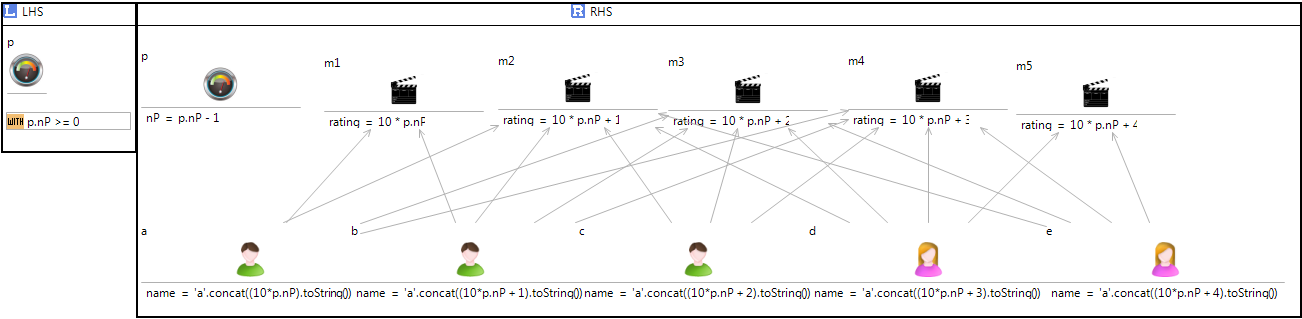
\includegraphics[width=\textheight, angle=90]{imgs/createPositiveRule}
  }
  \hfill
%  \subfloat[Rules' headers.]{
%    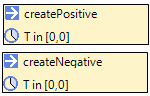
\includegraphics[width=0.2\textwidth]{imgs/headersCreate}
%  }
%  \hfill
  \subfloat[The \code{negativePositive} rule.\label{fig:createNegative}]{%
    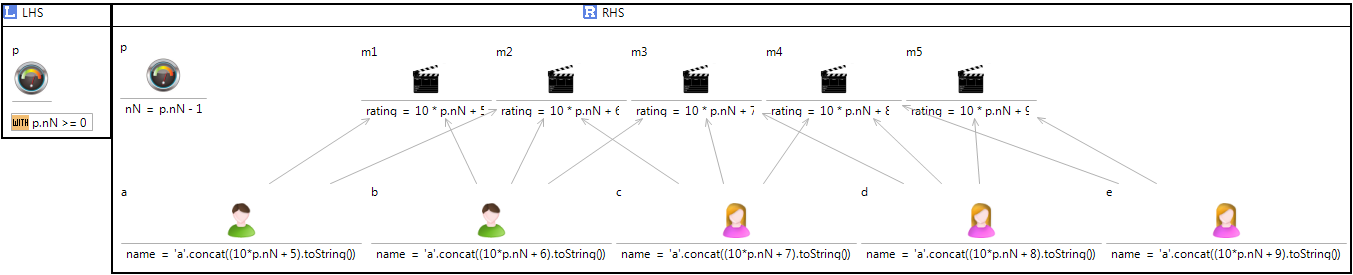
\includegraphics[width=\textheight, angle=90]{imgs/createNegativeRule}
  }
 
  \caption{Task 1 rules. \label{fig:task1}}
\end{figure}


